%!TEX TS-program = xelatex

% Шаблон документа LaTeX создан в 2018 году
% Алексеем Подчезерцевым
% В качестве исходных использованы шаблоны
% 	Данилом Фёдоровых (danil@fedorovykh.ru) 
%		https://www.writelatex.com/coursera/latex/5.2.2
%	LaTeX-шаблон для русской кандидатской диссертации и её автореферата.
%		https://github.com/AndreyAkinshin/Russian-Phd-LaTeX-Dissertation-Template

\documentclass[a4paper,14pt]{article}


%%% Работа с русским языком
\usepackage[english,russian]{babel}   %% загружает пакет многоязыковой вёрстки
\usepackage{fontspec}      %% подготавливает загрузку шрифтов Open Type, True Type и др.
\defaultfontfeatures{Ligatures={TeX},Renderer=Basic}  %% свойства шрифтов по умолчанию
\setmainfont[Ligatures={TeX,Historic}]{Times New Roman} %% задаёт основной шрифт документа
\setsansfont{Comic Sans MS}                    %% задаёт шрифт без засечек
\setmonofont{Courier New}
\usepackage{indentfirst}
\frenchspacing

\renewcommand{\epsilon}{\ensuremath{\varepsilon}}
\renewcommand{\phi}{\ensuremath{\varphi}}
\renewcommand{\kappa}{\ensuremath{\varkappa}}
\renewcommand{\le}{\ensuremath{\leqslant}}
\renewcommand{\leq}{\ensuremath{\leqslant}}
\renewcommand{\ge}{\ensuremath{\geqslant}}
\renewcommand{\geq}{\ensuremath{\geqslant}}
\renewcommand{\emptyset}{\varnothing}

%%% Дополнительная работа с математикой
\usepackage{amsmath,amsfonts,amssymb,amsthm,mathtools} % AMS
\usepackage{icomma} % "Умная" запятая: $0,2$ --- число, $0, 2$ --- перечисление

%% Номера формул
%\mathtoolsset{showonlyrefs=true} % Показывать номера только у тех формул, на которые есть \eqref{} в тексте.
%\usepackage{leqno} % Нумерация формул слева	

%% Перенос знаков в формулах (по Львовскому)
\newcommand*{\hm}[1]{#1\nobreak\discretionary{}
	{\hbox{$\mathsurround=0pt #1$}}{}}

%%% Работа с картинками
\usepackage{graphicx}  % Для вставки рисунков
\graphicspath{{images/}}  % папки с картинками
\setlength\fboxsep{3pt} % Отступ рамки \fbox{} от рисунка
\setlength\fboxrule{1pt} % Толщина линий рамки \fbox{}
\usepackage{wrapfig} % Обтекание рисунков текстом

%%% Работа с таблицами
\usepackage{array,tabularx,tabulary,booktabs} % Дополнительная работа с таблицами
\usepackage{longtable}  % Длинные таблицы
\usepackage{multirow} % Слияние строк в таблице
\usepackage{float}% http://ctan.org/pkg/float

%%% Программирование
\usepackage{etoolbox} % логические операторы


%%% Страница
\usepackage{extsizes} % Возможность сделать 14-й шрифт
\usepackage{geometry} % Простой способ задавать поля
\geometry{top=20mm}
\geometry{bottom=20mm}
\geometry{left=20mm}
\geometry{right=10mm}
%
%\usepackage{fancyhdr} % Колонтитулы
% 	\pagestyle{fancy}
%\renewcommand{\headrulewidth}{0pt}  % Толщина линейки, отчеркивающей верхний колонтитул
% 	\lfoot{Нижний левый}
% 	\rfoot{Нижний правый}
% 	\rhead{Верхний правый}
% 	\chead{Верхний в центре}
% 	\lhead{Верхний левый}
%	\cfoot{Нижний в центре} % По умолчанию здесь номер страницы

\usepackage{setspace} % Интерлиньяж
\onehalfspacing % Интерлиньяж 1.5
%\doublespacing % Интерлиньяж 2
%\singlespacing % Интерлиньяж 1

\usepackage{lastpage} % Узнать, сколько всего страниц в документе.

\usepackage{soul} % Модификаторы начертания

\usepackage{hyperref}
\usepackage[usenames,dvipsnames,svgnames,table,rgb]{xcolor}
\hypersetup{				% Гиперссылки
	unicode=true,           % русские буквы в раздела PDF
	pdftitle={Автоматизация проектных работ},   % Заголовок
	pdfauthor={Солодянкин А.А.},      % Автор
	pdfsubject={Автоматизация проектных работ},      % Тема
	pdfcreator={Солодянкин А.А.}, % Создатель
	pdfproducer={Солодянкин А.А.}, % Производитель
	pdfkeywords={Автоматизация проектных работ}, % Ключевые слова
	colorlinks=true,       	% false: ссылки в рамках; true: цветные ссылки
	linkcolor=black,          % внутренние ссылки
	citecolor=black,        % на библиографию
	filecolor=magenta,      % на файлы
	urlcolor=black           % на URL
}
\makeatletter 
\def\@biblabel#1{#1. } 
\makeatother
\usepackage{cite} % Работа с библиографией
%\usepackage[superscript]{cite} % Ссылки в верхних индексах
%\usepackage[nocompress]{cite} % 
\usepackage{csquotes} % Еще инструменты для ссылок

\usepackage{multicol} % Несколько колонок

\usepackage{tikz} % Работа с графикой
\usepackage{pgfplots}
\usepackage{pgfplotstable}

% ГОСТ заголовки
\usepackage[font=small]{caption}
%\captionsetup[table]{justification=centering, labelsep = newline} % Таблицы по правобу краю
%\captionsetup[figure]{justification=centering} % Картинки по центру


\newcommand{\tablecaption}[1]{\addtocounter{table}{1}\small \begin{flushright}\tablename \ \thetable\end{flushright}%	
\begin{center}#1\end{center}}

\newcommand{\imref}[1]{рис.~\ref{#1}}

\usepackage{multirow}
\usepackage{spreadtab}
\newcolumntype{K}[1]{@{}>{\centering\arraybackslash}p{#1cm}@{}}


\usepackage{xparse}
\usepackage{fancyvrb}

\RecustomVerbatimCommand{\VerbatimInput}{VerbatimInput}
{
	fontsize=\footnotesize    
}

\newcolumntype{?}[1]{!{\vrule width #1}}

\usepackage{tocloft}
\renewcommand{\cftsecleader}{\cftdotfill{\cftdotsep}}
\begin{document} % конец преамбулы, начало документа
\begin{titlepage}
	\begin{center}
		ПРАВИТЕЛЬСТВО РОССИЙСКОЙ ФЕДЕРАЦИИ \\
 		ФЕДЕРАЛЬНОЕ  ГОСУДАРСТВЕННОЕ АВТОНОМНОЕ \\
		ОБРАЗОВАТЕЛЬНОЕ УЧРЕЖДЕНИЕ ВЫСШЕГО ОБРАЗОВАНИЯ\\
		«НАЦИОНАЛЬНЫЙ ИССЛЕДОВАТЕЛЬСКИЙ УНИВЕРСИТЕТ\\
		«ВЫСШАЯ ШКОЛА ЭКОНОМИКИ»
	\end{center}
	
	\begin{center}
		\textbf{Московский институт электроники и математики}
		
		\textbf{Им. А.Н.Тихонова НИУ ВШЭ}
		
		\vspace{2ex}
		
		\textbf{Департамент компьютерной инженерии}
	\end{center}
	\vspace{1ex}	
	
	\vspace{1ex}
	\begin{center}
		\textbf{Практическая работа №4 \\
			«Знакомство с САПР Altera Quartus II» \\
			Вариант №13
	}
	\end{center}	

	\vspace{2ex}
	\vfill
	
	\vspace{2ex}
	
	\begin{flushright}
		\textbf{Выполнил:}
		
		\vspace{2ex}
		
		Студент группы БИВ174
		
		\vspace{2ex}
		
		Солодянкин Андрей Александрович
		
		\vspace{2ex}
		
		\textbf{Проверил:}
		
		\vspace{2ex}
		
		Романова Ирина Ивановна
	\end{flushright}

	\vspace{5ex}
	\begin{center}
		Москва \the\year \, г.
	\end{center}
	
\end{titlepage}
\addtocounter{page}{1}

\tableofcontents
\pagebreak

\section{Цель работы}

Моделирование работы дешифратора, изучение карт Карно.

\section{Задание}

\begin{enumerate}
\item Используя логические элементы спроектировать схему и исследовать работу (снять временную характеристику и таблицу задержек) одноразрядного двухразрядного и четырехразрядного сумматора.

\item Построить временную диаграмму и выполнить моделирование в режимах Functional и Time. Сравнить и обосновать полученные результаты.

\item Запрограммировать учебную плату и продемонстрировать результаты работы на макете.

\item На базе сумматора построить вычитатель. Спроектировать его схему и исследовать работу (снять временную диаграмму и таблицу задержек)

\item Построить временную диаграмму и выполнить моделирование в режимах Functional и Time. Сравнить и обосновать полученные результаты.

\item Запрограммировать учебную плату и продемонстрировать результаты работы на макете.
\end{enumerate}

\section{Выполнение работы}

\subsection{Исследование сумматоров}

\subsubsection{Проектирование одноразрядного сумматора}

Построим схему одноразрядного сумматора (рис. \ref{fig:041bdf}).

\begin{figure}[H]
	\centering
	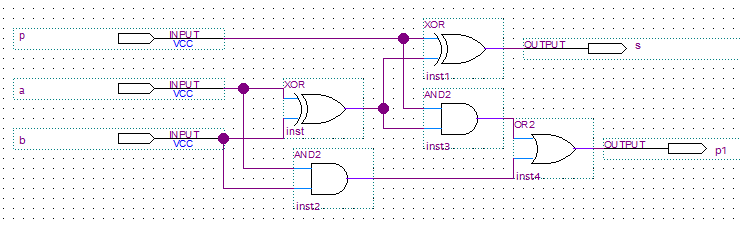
\includegraphics[width=0.7\linewidth]{image/04_1_bdf}
	\caption{Схема одноразрядного сумматора}
	\label{fig:041bdf}
\end{figure}


Для одноразрядного сумматора получились следующие задержки (рис. \ref{fig:041time}). Временные задержки были получены следующим образом: TimeQuest Timing Analysis > Write SDC file.. > Report Datasheet.

\begin{figure}[H]
	\centering
	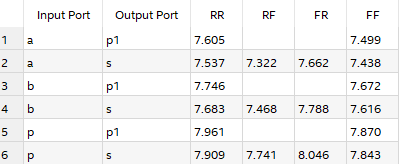
\includegraphics[width=0.7\linewidth]{image/04_1_time}
	\caption{Временные задержки одноразрядного сумматора}
	\label{fig:041time}
\end{figure}

В файле с временными диаграммами добавим все пины и установим входные значения. Полученные временные диаграммы рис. \ref{fig:041wvf}.

\begin{figure}[H]
	\centering
	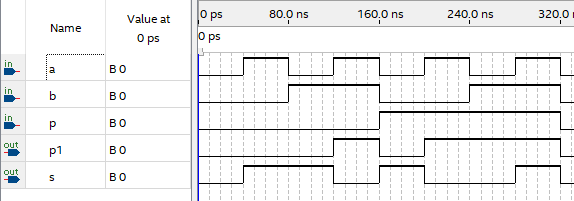
\includegraphics[width=0.9\linewidth]{image/04_1_wvf}
	\caption{Временные диаграммы одноразрядного сумматора}
	\label{fig:041wvf}
\end{figure}

 Моделирование в режимах Functional и Time не отличается, т.к. на приведенной частоте задержек не видно.
 
 Загрузим на плату и протестируем работу (рис. \ref{fig:041foto})
 
 \begin{figure}[H]
 	\centering
 	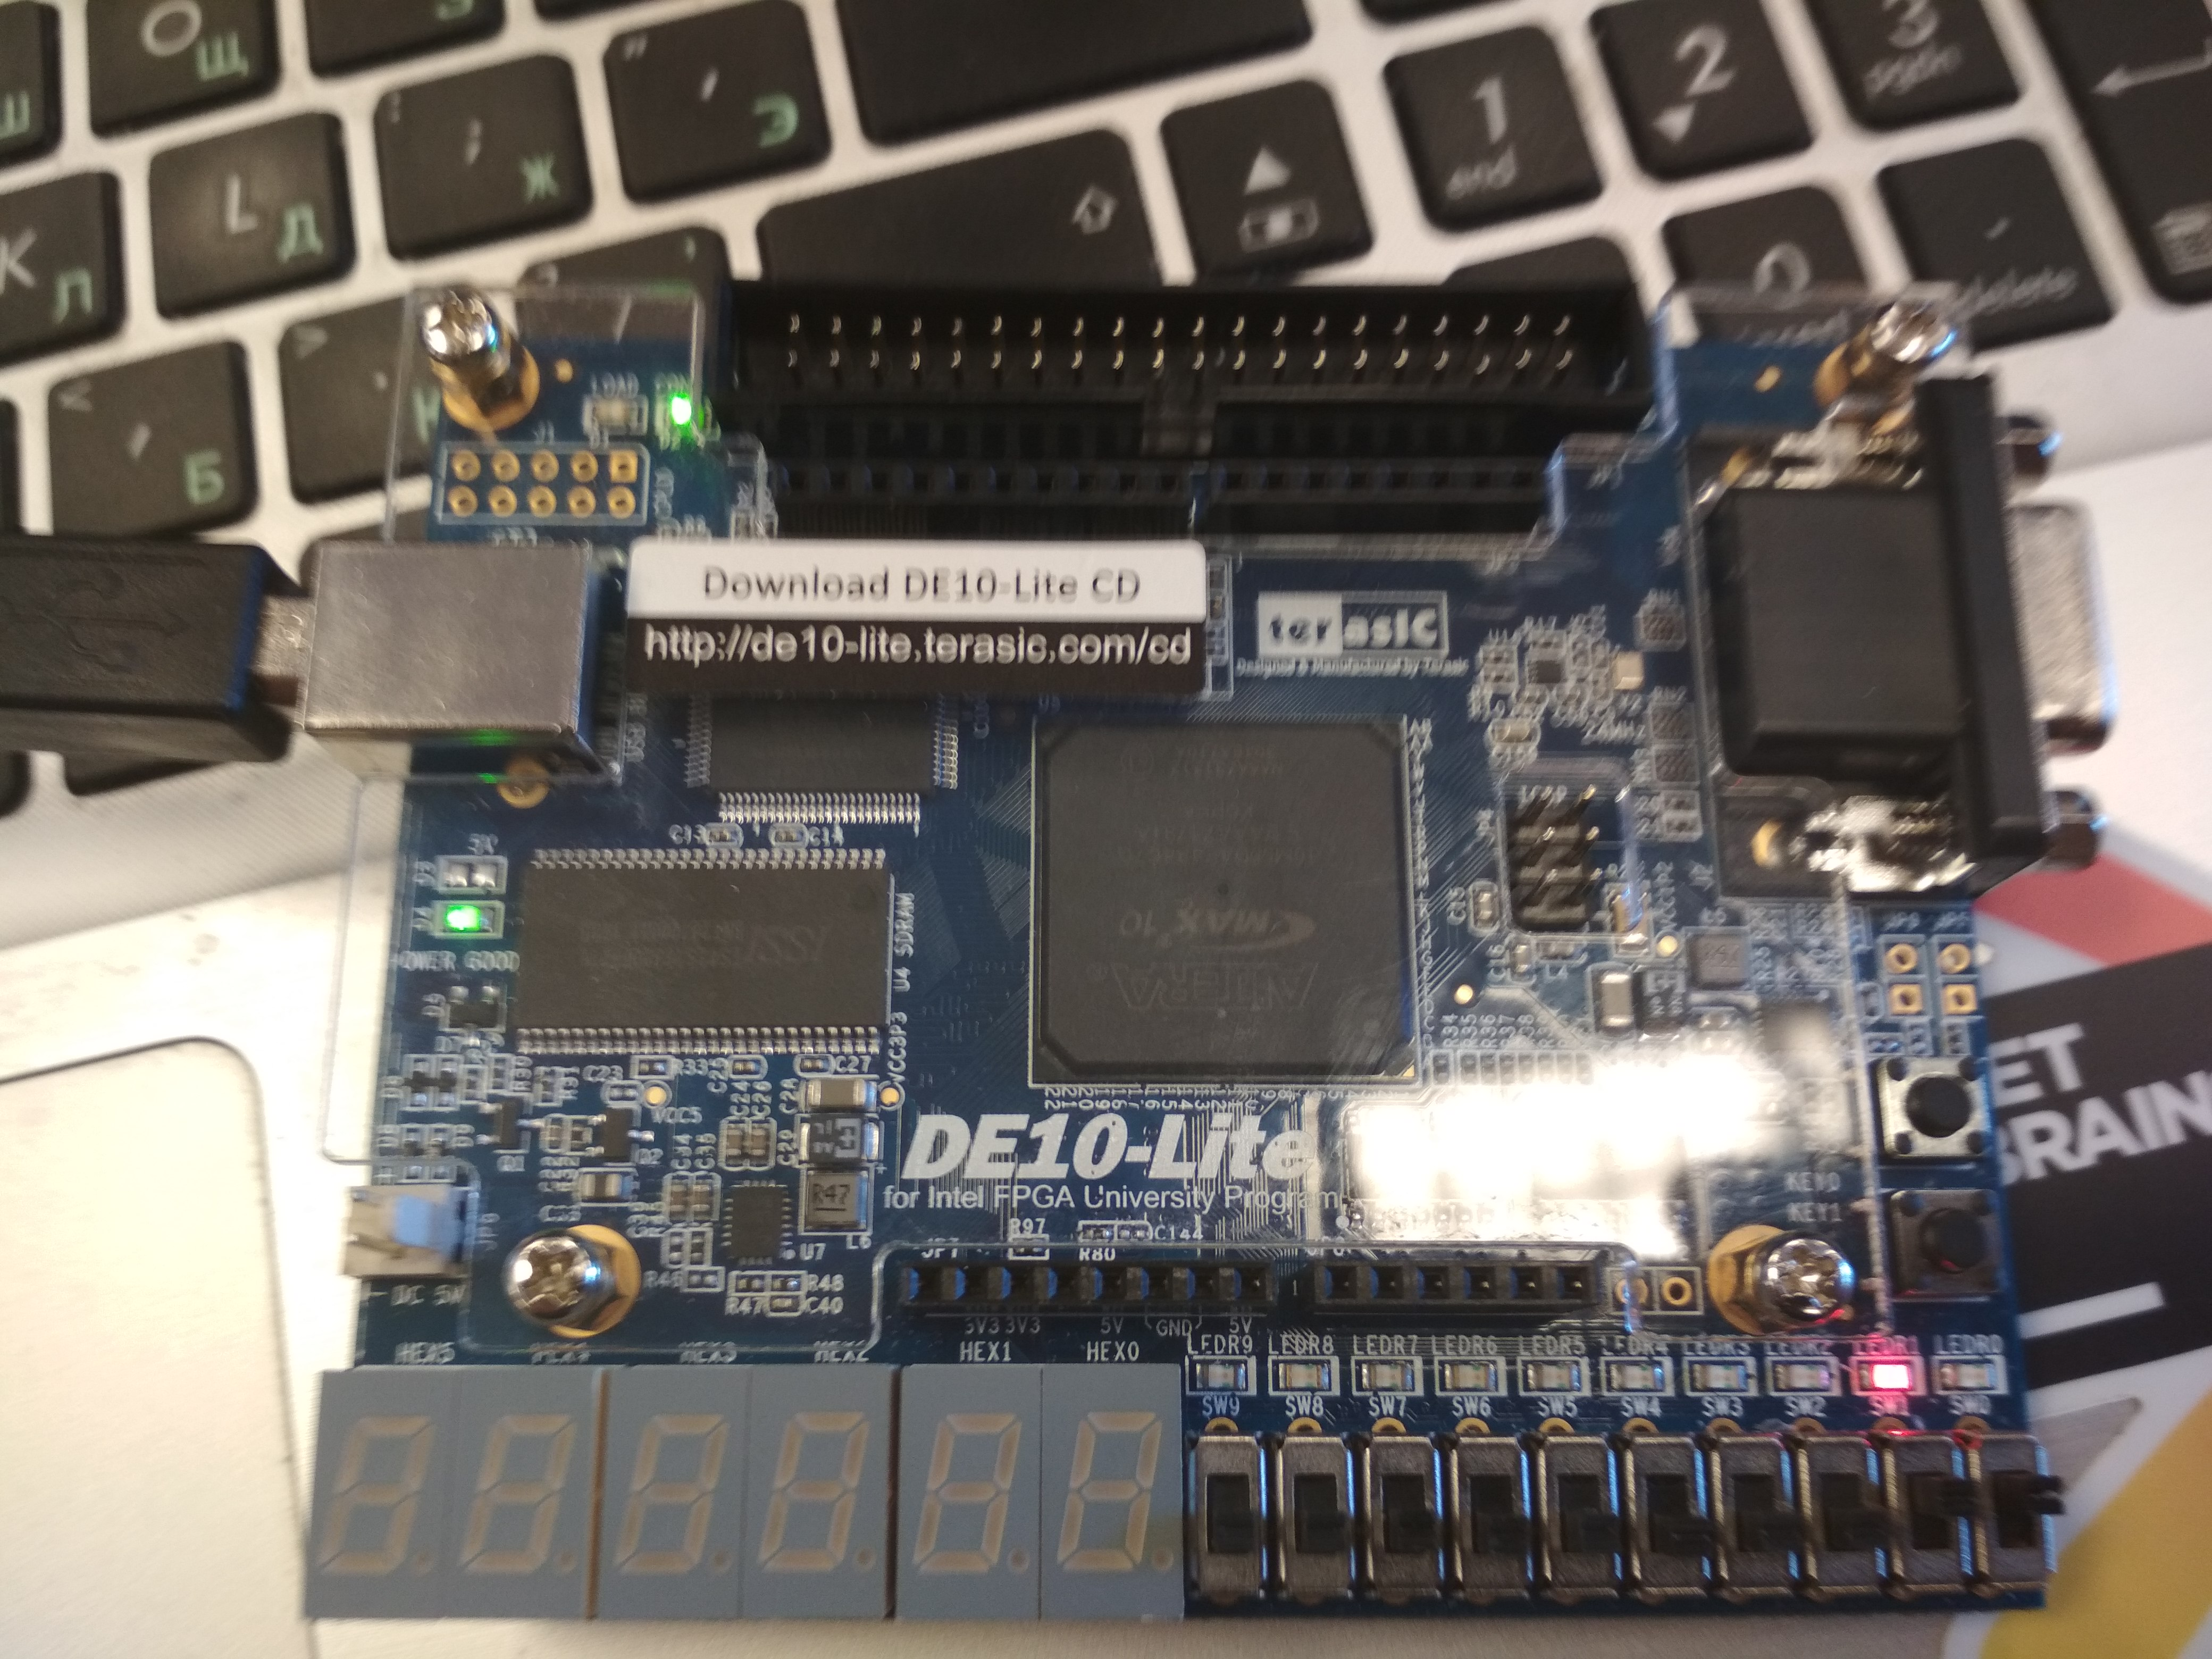
\includegraphics[width=0.7\linewidth]{image/lab4/2020-03-1412-17-02.JPG}
 	\caption{Фото рабочей платы}
 	\label{fig:041foto}
 \end{figure}

(Фото есть т.к. работа выполнялась до карантина)

Далее соберем данную схему как один логический элемент. Для этого необходимо выбрать в меню File Create/Update, далее Create Symbol Files for Current File (рис. \ref{fig:04createsymbol}).

\begin{figure}[H]
	\centering
	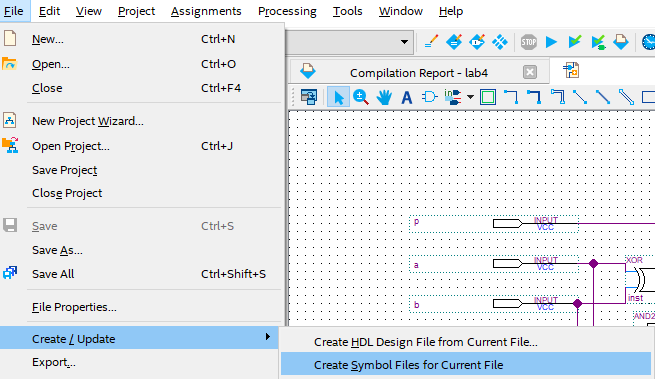
\includegraphics[width=0.7\linewidth]{image/04_create_symbol}
	\caption{Создание логического элемента}
	\label{fig:04createsymbol}
\end{figure}

В открывшемся окне сохраняем элемент.

\subsubsection{Исследование работы двухразрядного сумматора}

В меню логических элементов найдем созданный нами одноразрядный сумматор. На его основе спроектируем двухразрядный сумматор (рис. \ref{fig:042sumbdf}).

\begin{figure}[H]
	\centering
	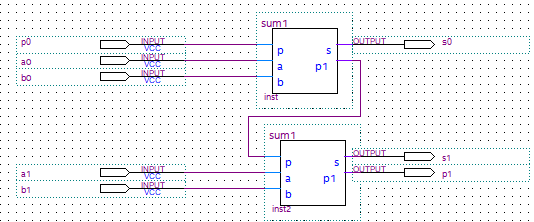
\includegraphics[width=0.7\linewidth]{image/lab4/04_2sum_bdf}
	\caption{Схема двухразрядного сумматора}
	\label{fig:042sumbdf}
\end{figure}

По описанному ранее порядку найдем временные задержки (рис. \ref{fig:042sumtime}).

\begin{figure}[H]
	\centering
	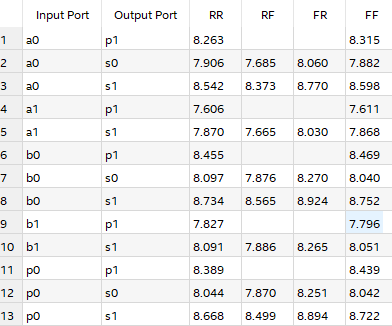
\includegraphics[width=0.7\linewidth]{image/lab4/04_2sum_time}
	\caption{Временные задержки двухразрядного сумматора}
	\label{fig:042sumtime}
\end{figure}

В результате моделирования временная диаграмма имеет следующий вид (рис. \ref{fig:042sumwvf}).

\begin{figure}[H]
	\centering
	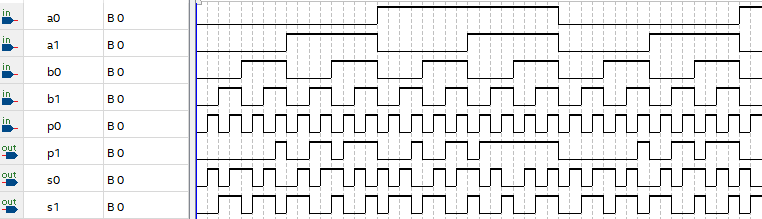
\includegraphics[width=0.9\linewidth]{image/lab4/04_2sum_wvf}
	\caption{Временная диаграмма для двухразрядного сумматора}
	\label{fig:042sumwvf}
\end{figure}

 Моделирование в режимах Functional и Time не отличается, т.к. на приведенной частоте задержек не видно.
 
 Загрузим на плату и протестируем работу (рис. \ref{fig:042foto})
 
 \begin{figure}[H]
 	\centering
 	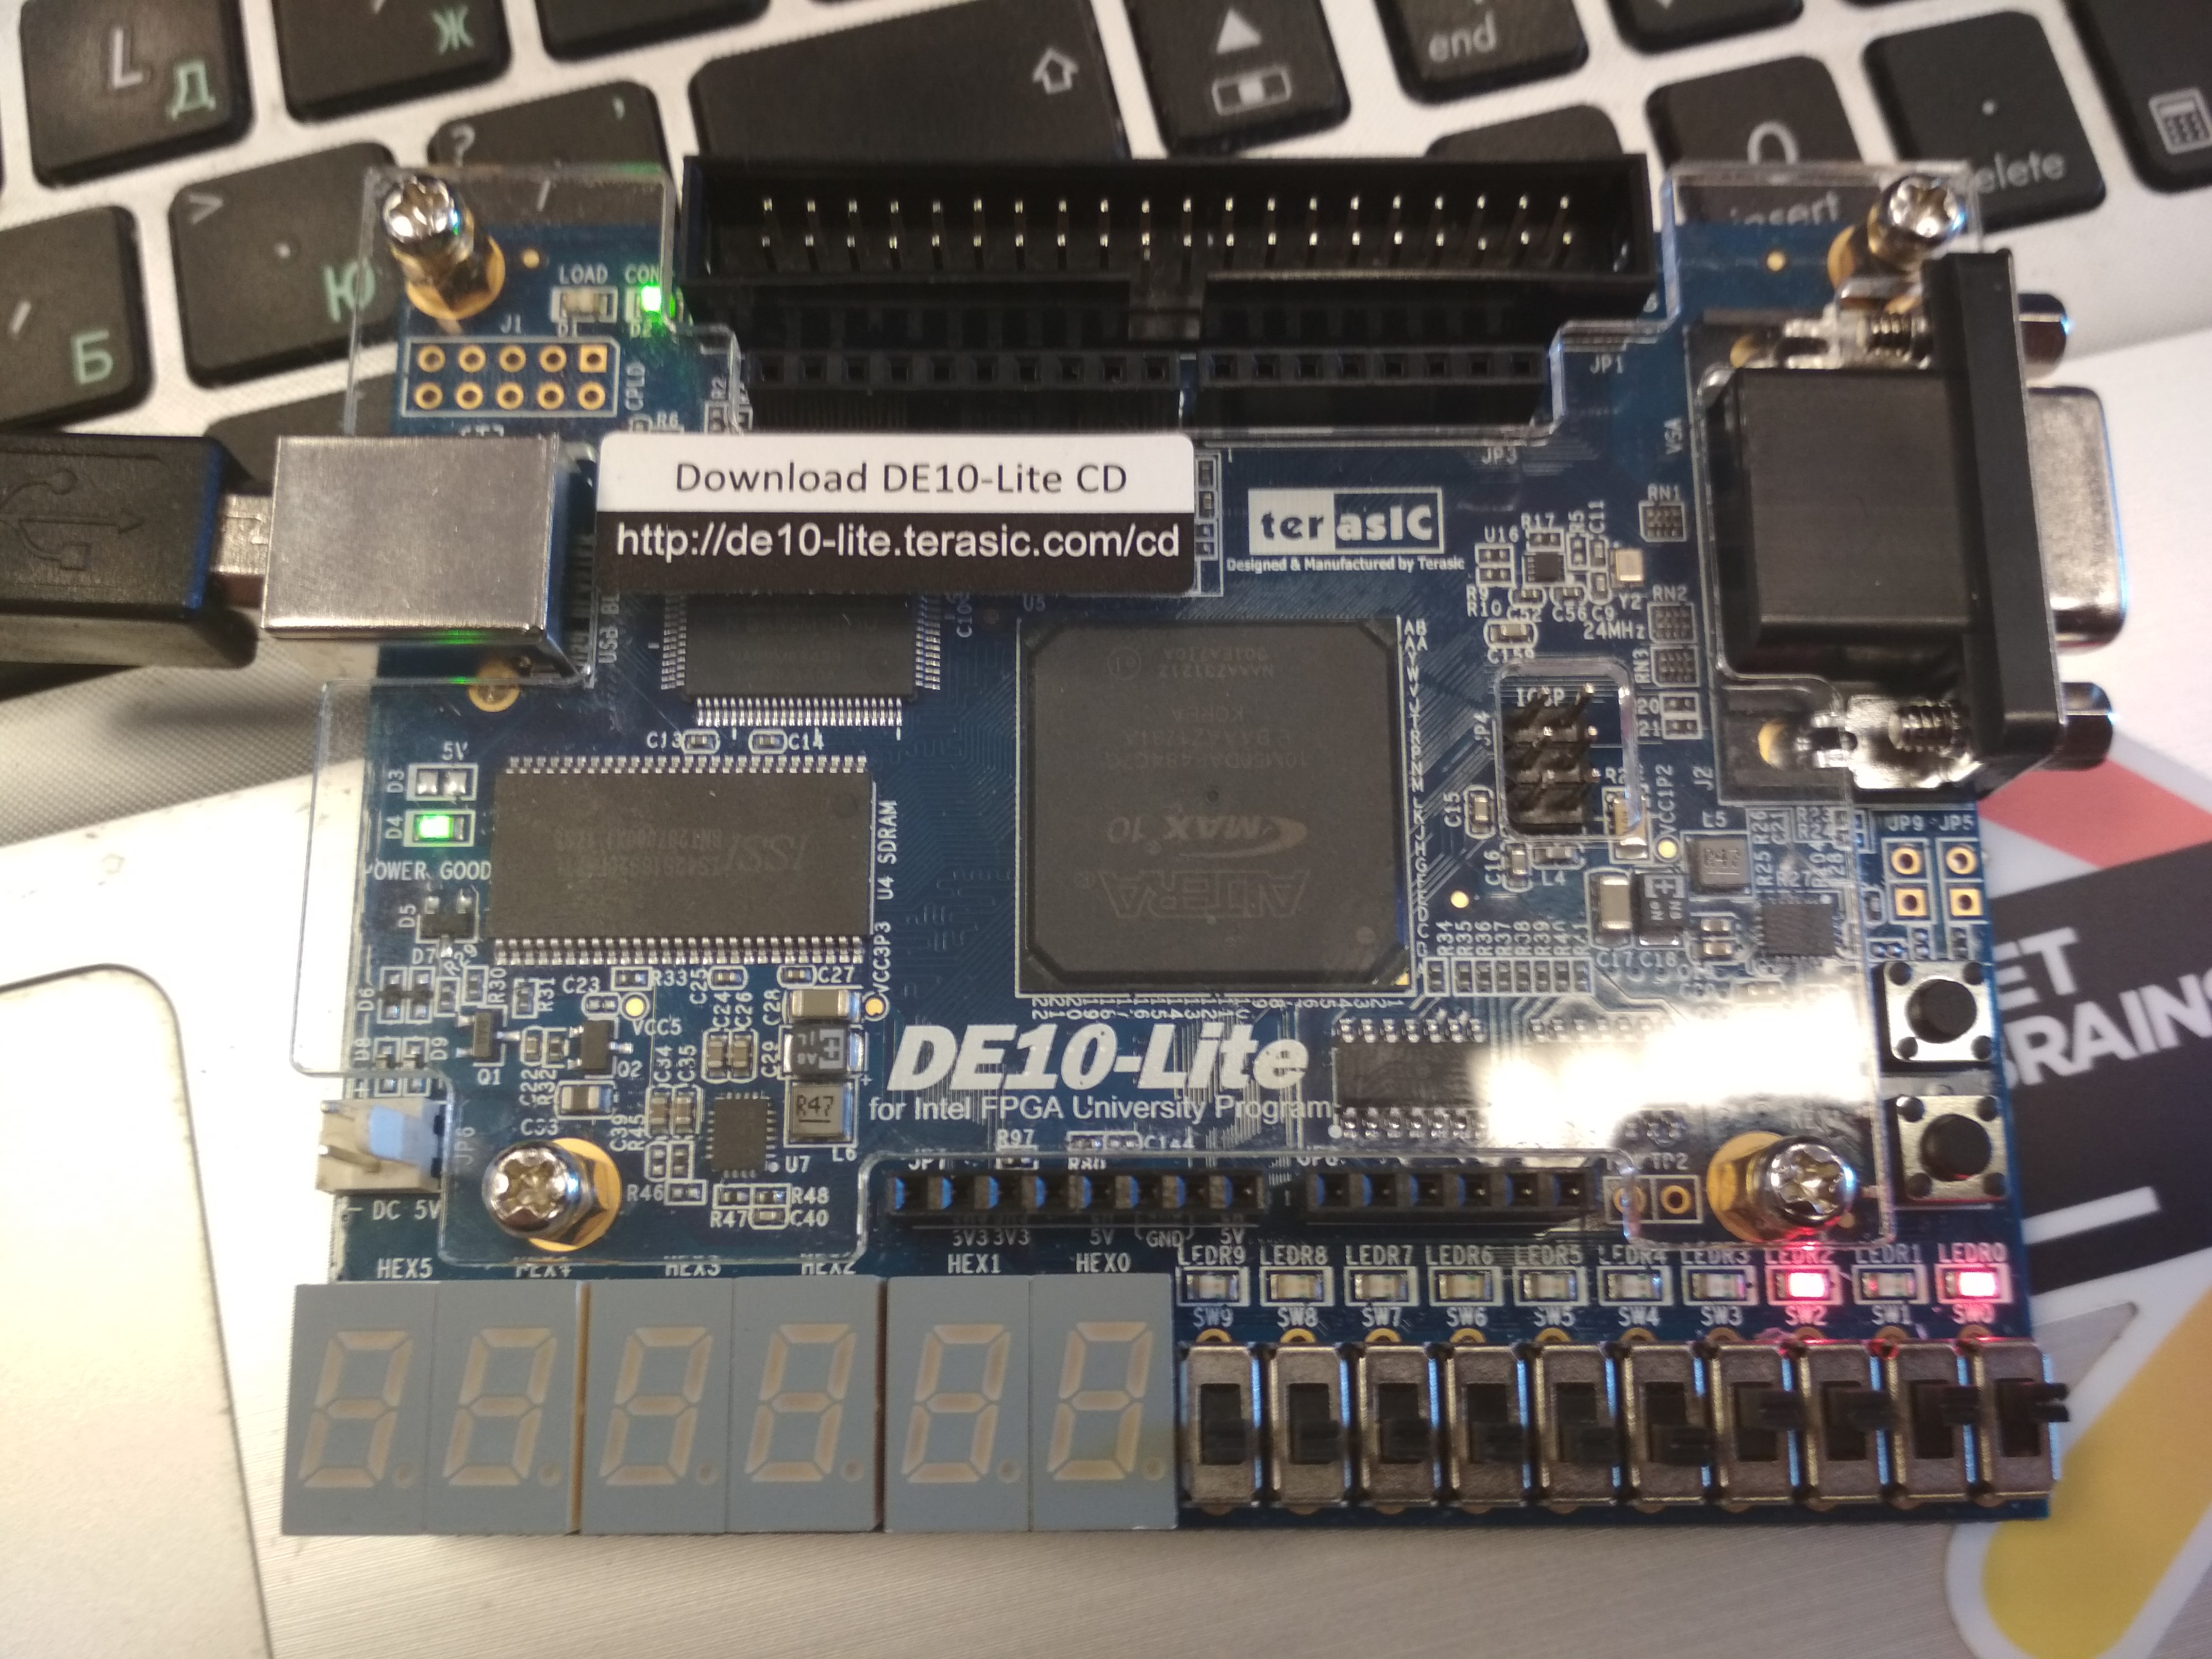
\includegraphics[width=0.7\linewidth]{image/lab4/2020-03-1412-17-16.JPG}
 	\caption{Фото рабочей платы}
 	\label{fig:042foto}
 \end{figure}

\subsubsection{Исследование работы четырехразрядного сумматора}

В меню логических элементов найдем созданный нами одноразрядный сумматор. На его основе спроектируем четырехразрядный сумматор (рис. \ref{fig:044sumbdf}).

\begin{figure}[H]
	\centering
	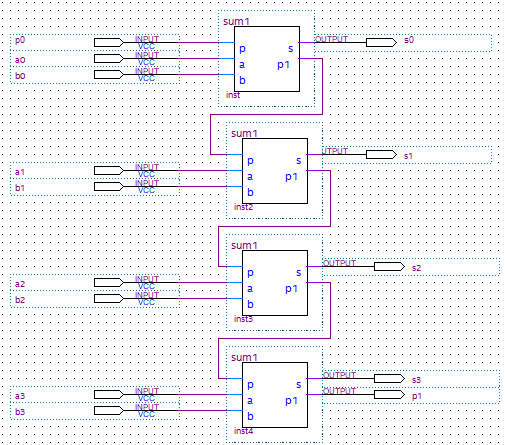
\includegraphics[width=0.7\linewidth]{image/lab4/04_4sum_bdf}
	\caption{Схема четырехразрядного сумматора}
	\label{fig:044sumbdf}
\end{figure}

По описанному ранее порядку найдем временные задержки (рис. \ref{fig:044sumtime}).

\begin{figure}[H]
	\centering
	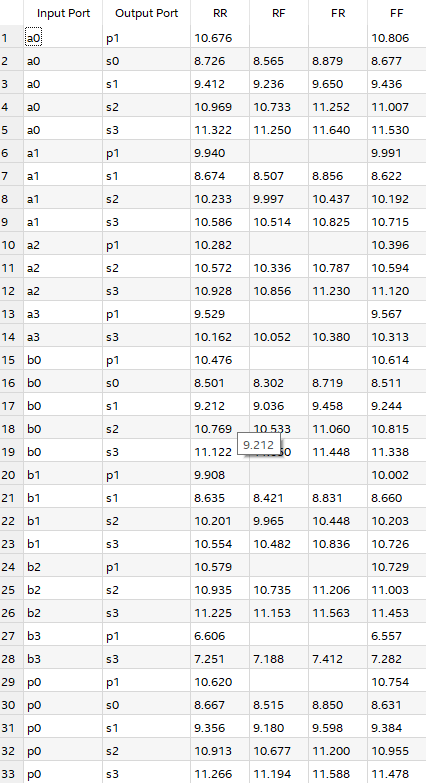
\includegraphics[width=0.7\linewidth]{image/lab4/04_4sum_time}
	\caption{Временные задержки четырехразрядного сумматора}
	\label{fig:044sumtime}
\end{figure}


В результате моделирования временная диаграмма имеет следующий вид (рис. \ref{fig:044sumwvf}).

\begin{figure}[H]
	\centering
	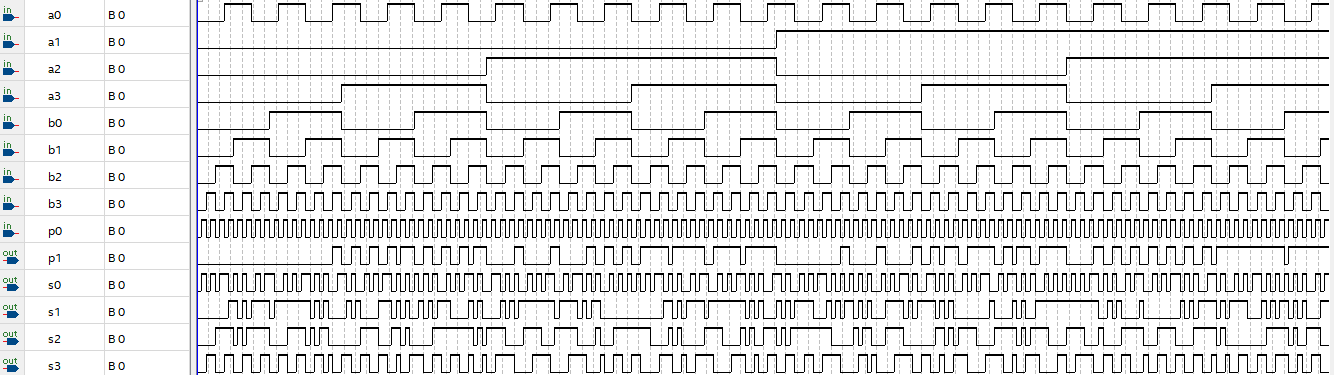
\includegraphics[width=0.9\linewidth]{image/lab4/04_4sum_wvf}
	\caption{Временная диаграмма для четырехразрядного сумматора}
	\label{fig:044sumwvf}
\end{figure}

Моделирование в режимах Functional и Time не отличается, т.к. на приведенной частоте задержек не видно.

Загрузим на плату и протестируем работу (рис. \ref{fig:044foto})

\begin{figure}[H]
	\centering
	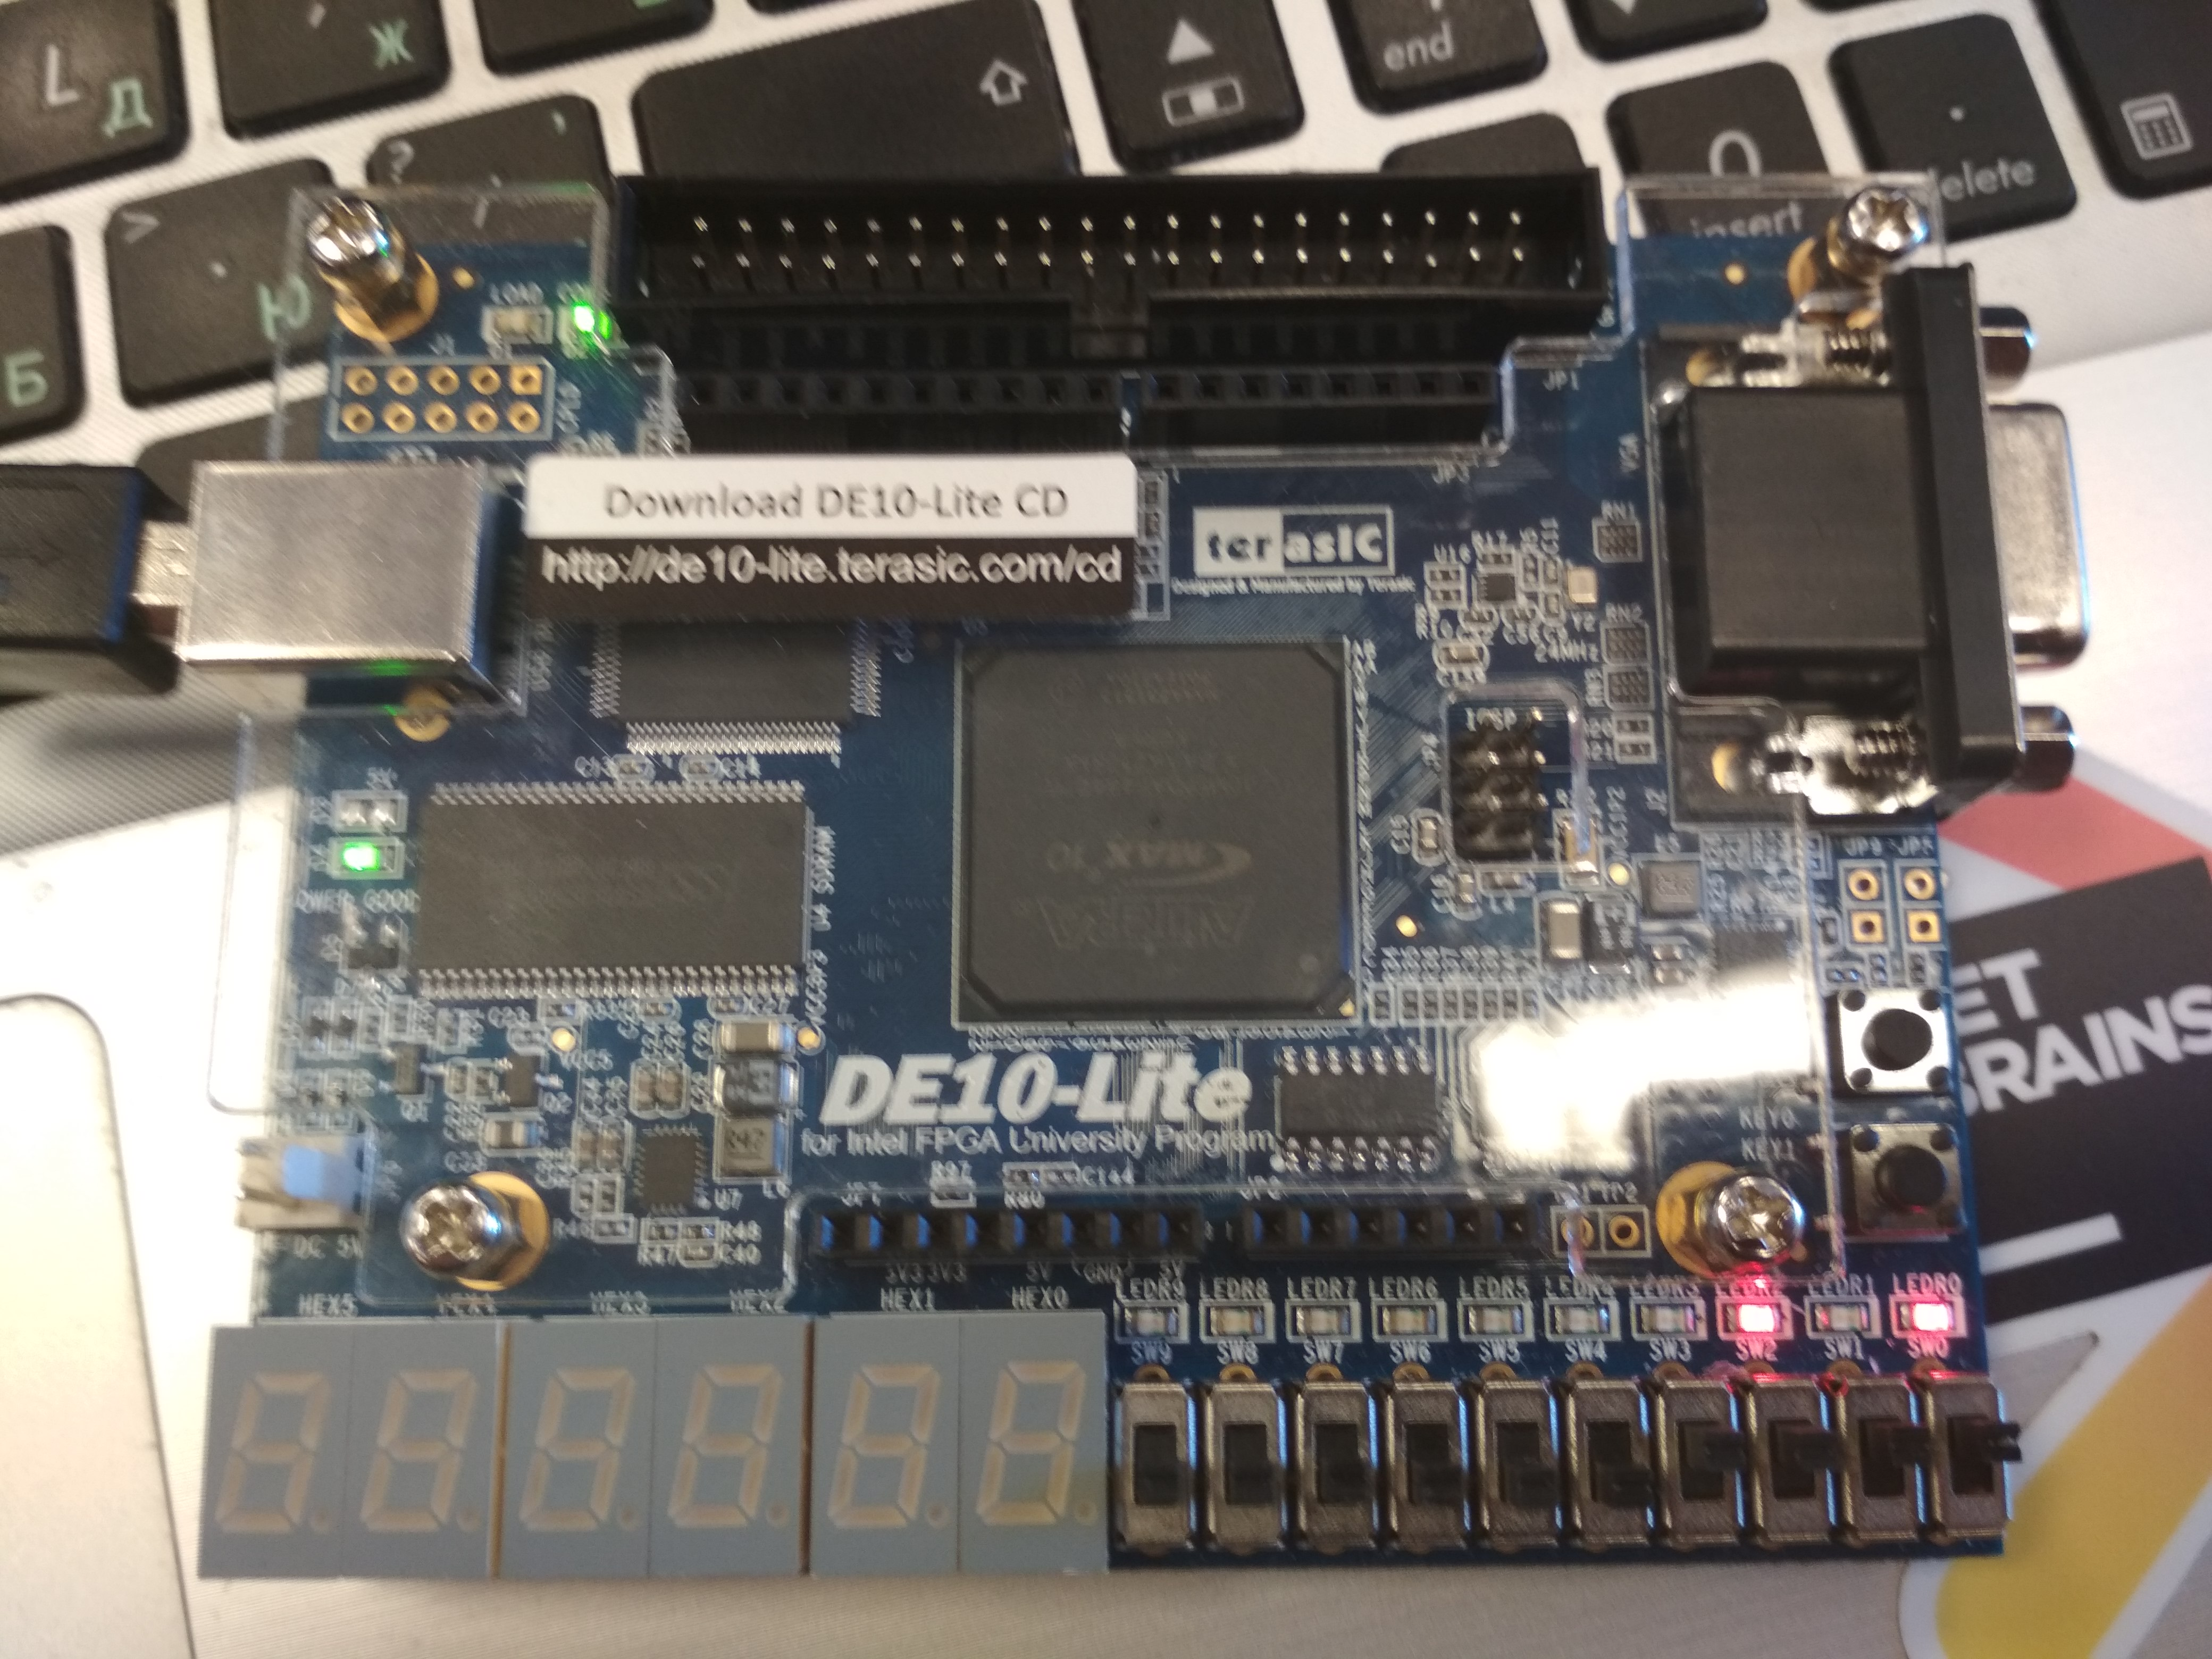
\includegraphics[width=0.7\linewidth]{image/lab4/2020-03-1412-17-14.JPG}
	\caption{Фото рабочей платы}
	\label{fig:044foto}
\end{figure}

\subsection{Исследование работы четырехразрядного вычитателя}

Есть 2 числа $A = a_3a_2a_1a_0$ и $B = b_3b_2b_1b_0$, необходимо получить разность чисел $B$ и $A$ $S = s_3s_2s_1s_0$. $p$ - сигнал переполнения.

Для реализации вычитателя необходимо инвертировать вычитаемое число и вход переноса из предыдущего разряда подать логическую единицу.

В меню логических элементов найдем созданный нами одноразрядный сумматор. На его основе спроектируем четырехразрядный вычитатель (рис. \ref{fig:044vicbdf}).

\begin{figure}[H]
	\centering
	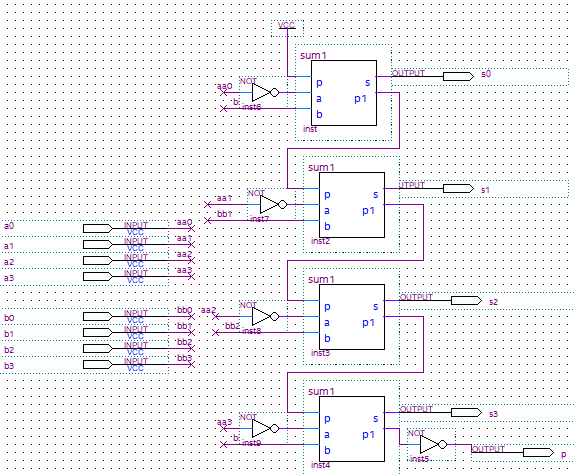
\includegraphics[width=0.7\linewidth]{image/lab4/04_4vic_bdf}
	\caption{Схема четырехразрядного вычитателя}
	\label{fig:044vicbdf}
\end{figure}


По описанному ранее порядку найдем временные задержки (рис. \ref{fig:044victime}).

\begin{figure}[H]
	\centering
	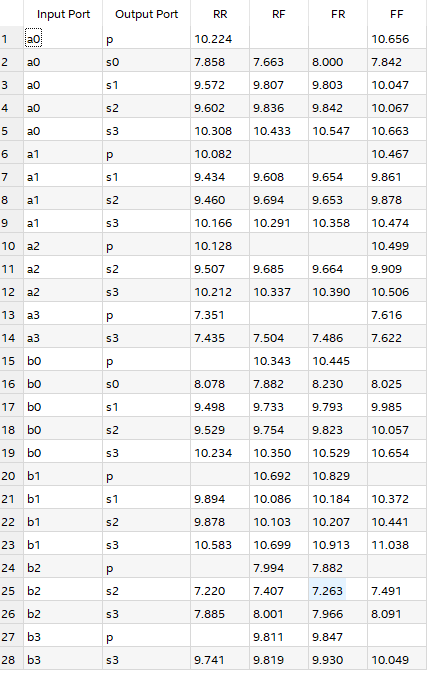
\includegraphics[width=0.7\linewidth]{image/lab4/04_4vic_time}
	\caption{Временные задержки четырехразрядного вычитателя}
	\label{fig:044victime}
\end{figure}

В результате моделирования временная диаграмма имеет следующий вид (рис. \ref{fig:044vicwvf}).

\begin{figure}[H]
	\centering
	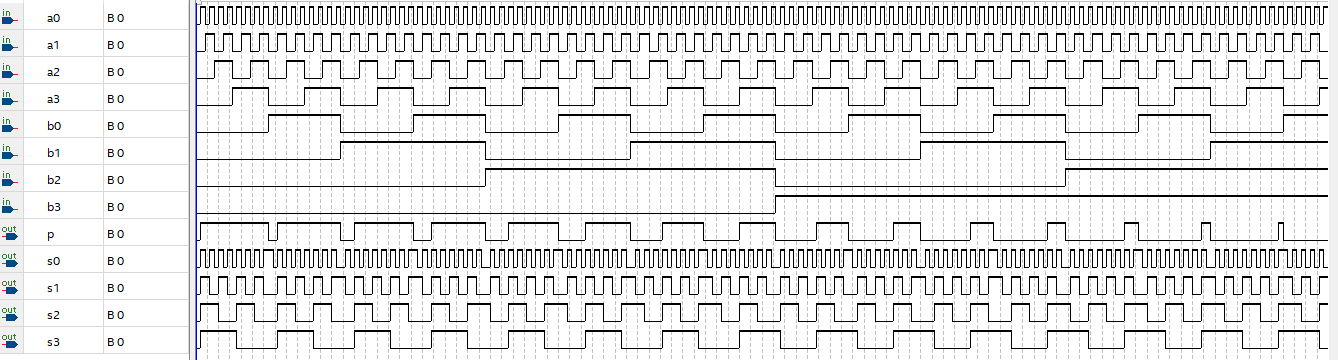
\includegraphics[width=0.9\linewidth]{image/lab4/04_4vic_wvf}
	\caption{Временная диаграмма для четырехразрядного вычитателя}
	\label{fig:044vicwvf}
\end{figure}


Моделирование в режимах Functional и Time не отличается, т.к. на приведенной частоте задержек не видно.

Загрузим на плату и протестируем работу (рис. \ref{fig:044vicfoto})

\begin{figure}[H]
	\centering
	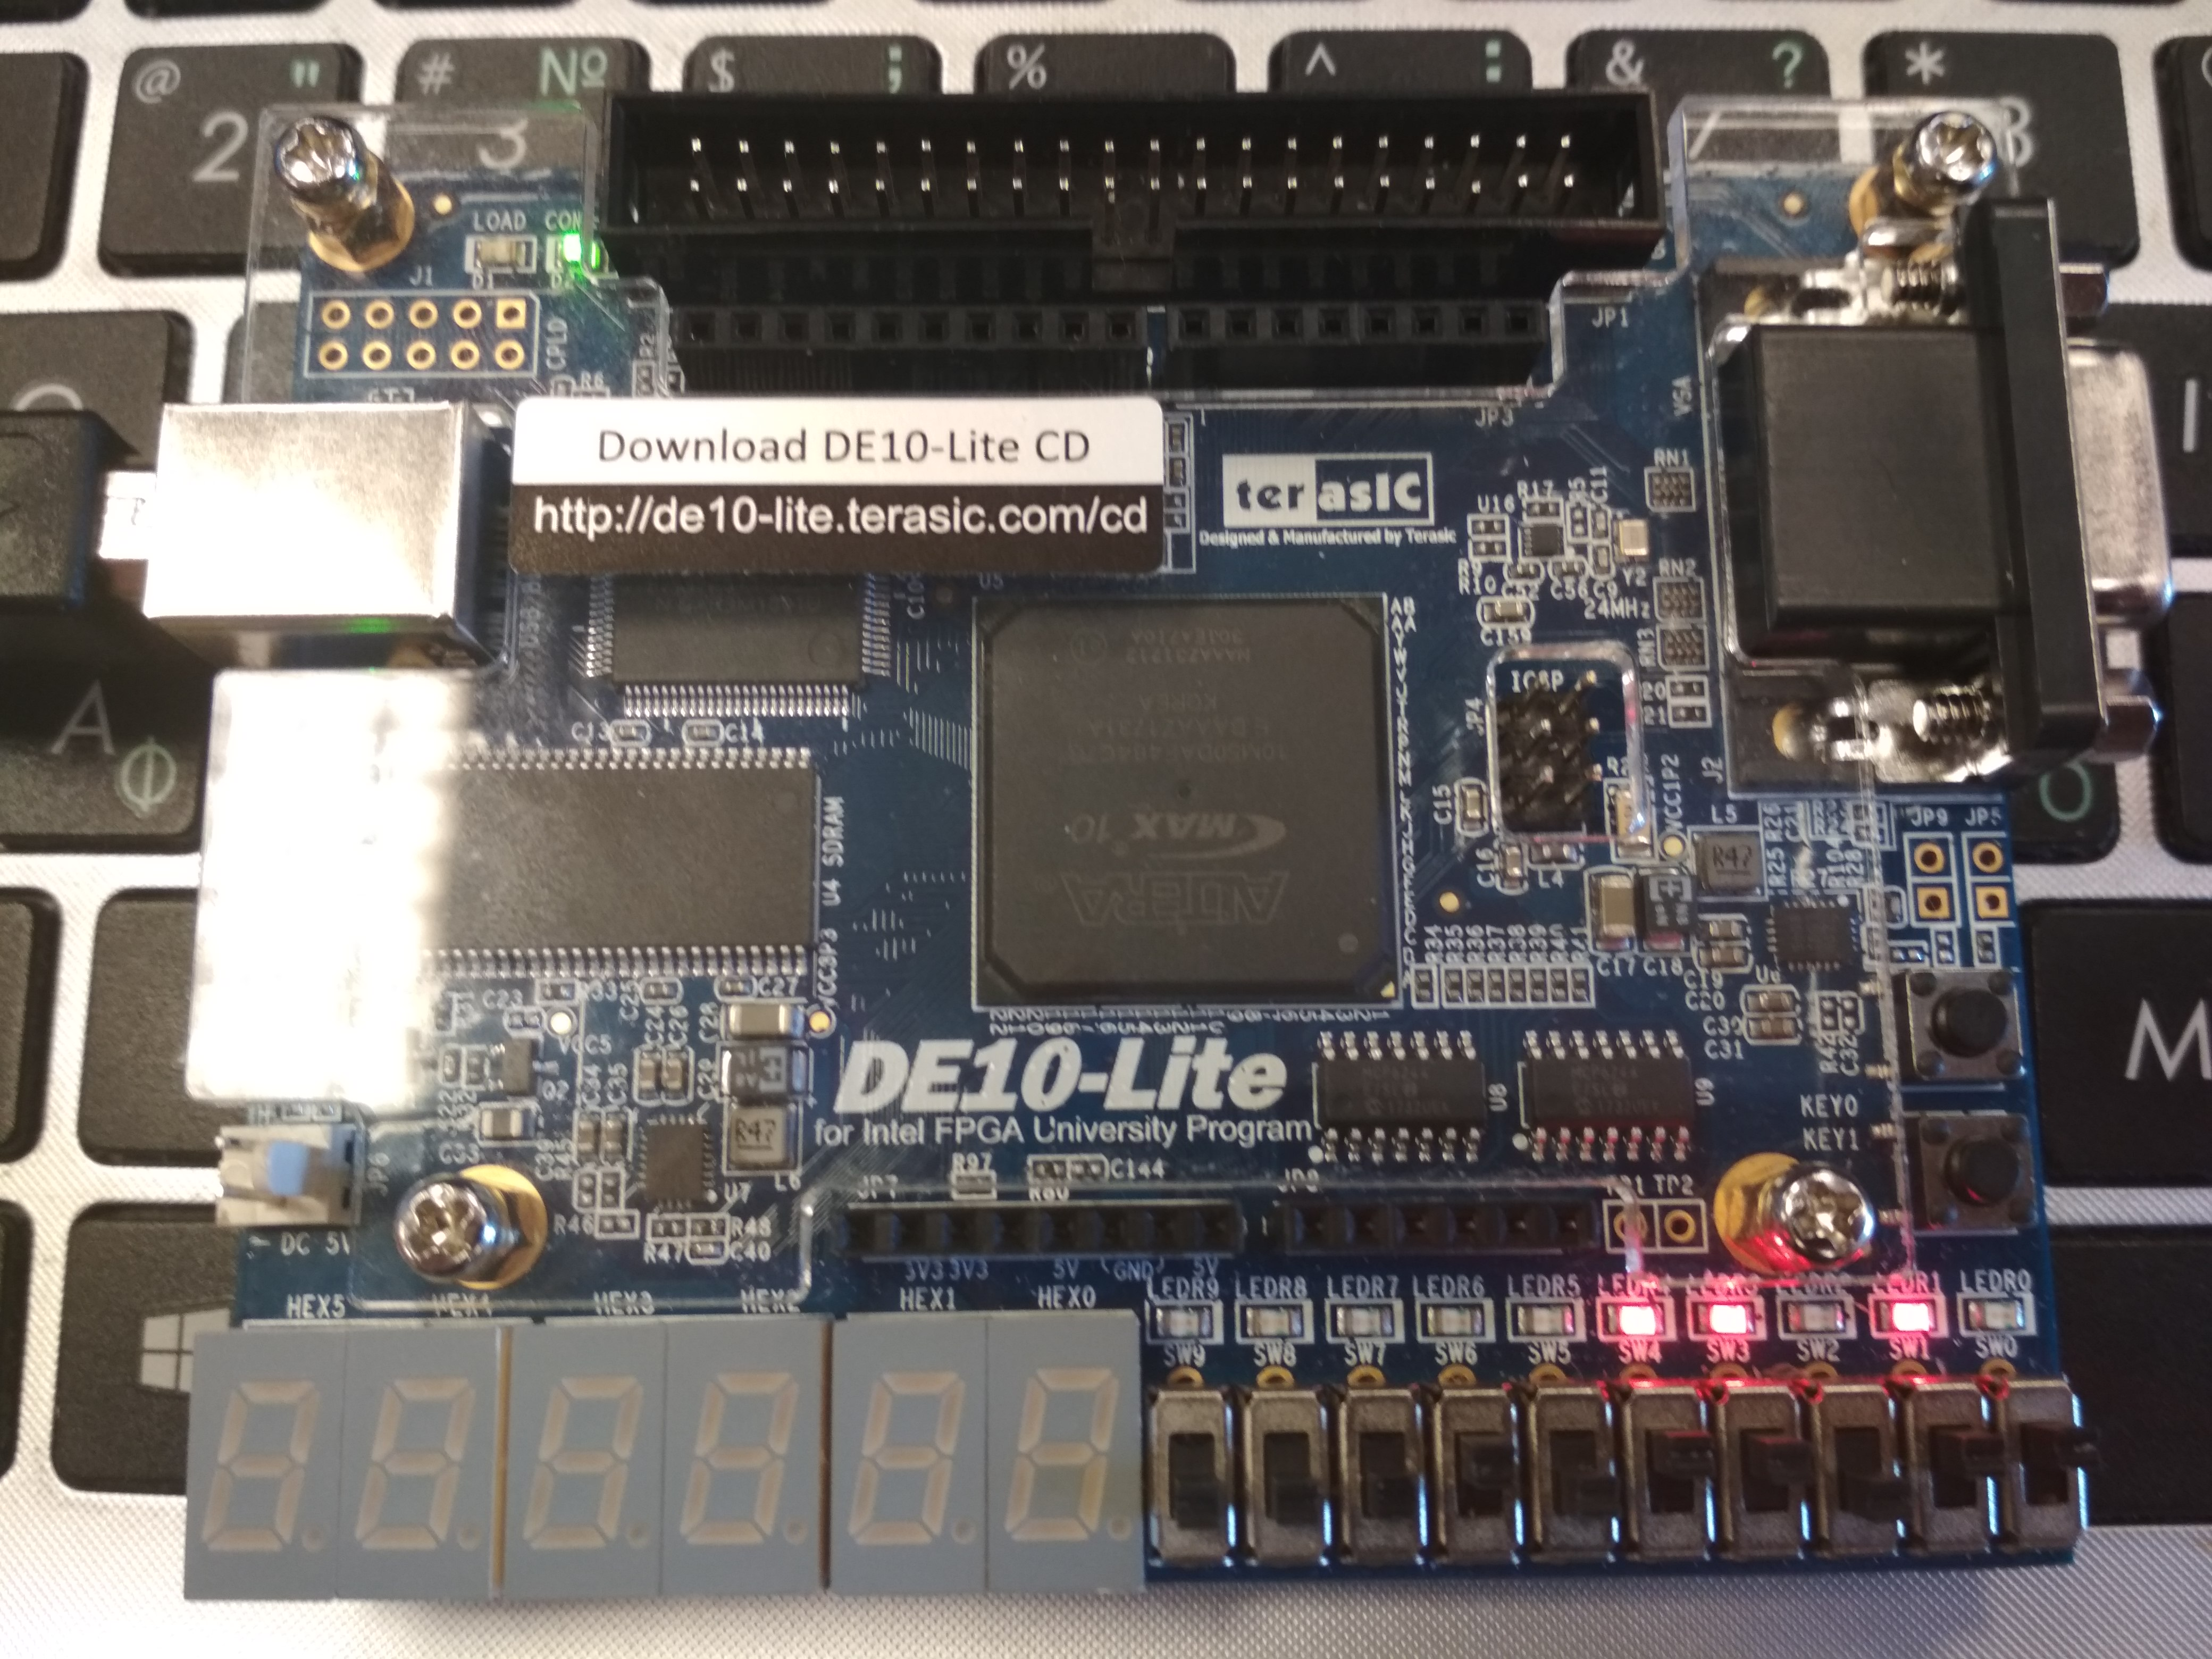
\includegraphics[width=0.7\linewidth]{image/lab4/2020-03-1413-07-27.JPG}
	\caption{Фото рабочей платы}
	\label{fig:044vicfoto}
\end{figure}

\section{Вывод}
В ходе проделанной работы был создан одноразрядный сумматор.
На его основе были спроектированы двухразрядный и четырехразрядный сумматоры, а также четырехразрядный вычитатель.
При помощи TimeQuest Timing Analysis были получены задержки для кажого входного параметра.
Схема была протестированы при помощи WaveForm, а также удалось загрузить схему на плату и протестировать работоспособность программы на плате.

\newpage 
\renewcommand{\refname}{{\normalsize СПИСОК ИСПОЛЬЗОВАННЫХ ИСТОЧНИКОВ}} 
\centering 
\begin{thebibliography}{9} 
	\addcontentsline{toc}{section}{\refname} 
	\bibitem{sql} Vijayakumar P., Vijayalakshmi V., Zayaraz G. Comparative study of hyperelliptic curve cryptosystem over prime field and its survey //International Journal of Hybrid Information Technology. – 2014. – Т. 7. – №. 1. – С. 137-146.
	\bibitem{sql} Антонов А., Филиппов А., Золотухо Р. Средства системной отладки САПР Quartus II //Компоненты и технологии. – 2008. – №. 89.
\end{thebibliography}

\end{document} % конец документа